\documentclass[11pt]{article}

% Pacotes extras necessários
\usepackage{amsmath}
\usepackage[lmargin=0.7in, rmargin=0.7in, tmargin=0.5in, bmargin=0.5in, includehead, includefoot]{geometry}
\usepackage{amsfonts}
\usepackage[utf8]{inputenc}
\usepackage[portuguese]{babel}
\usepackage{graphicx}
\usepackage{fancyhdr}
\usepackage{setspace}

\graphicspath{ {./images/} }

% Sets para outras partes
\setlength{\parindent}{0pt}
\setstretch{1.25}
\DeclareMathOperator{\sen}{sen}

%% Facilidades
%% -- Laplace
\newcommand{\Lap}[1]{\mathcal{L}\left\{#1\right\}}

%% -- Fourier
\newcommand{\Fou}[1]{\mathcal{F}\left\{#1\right\}}

% ------- Estilo do trabalho -------- %
\fancypagestyle{capa}{
    \fancyhf{}
    \renewcommand\headrulewidth{0pt}
    \fancyfoot[C]{
        Rio de Janeiro\\
        2022
    }
}

\pagestyle{fancy}
\fancyhead{}
\fancyhead[L]{\thepage}
\fancyfoot{}
% ----------------------------------- %

% Dados do Grupo
\title{Sinais e Sistemas - Trabalho 4 - Avaliação 8}
\author{
    \textbf{Grupo 2}\\
    Leonardo Soares da Costa Tanaka\\
    Matheus Henrique Sant Anna Cardoso\\
    Theo Rudra Macedo e Silva
}
\date{}

\begin{document}
\maketitle
\thispagestyle{capa}
\newpage

\textbf{1.) Abaixo, use o número do grupo como o valor do parâmetro $p$. Entre no Octave com \texttt{B = [0 ; 0 ; 1], C = [1 0 0], A = [0 1 0 ; 0 0 1 ; (-2p) (-2p + 2) (-p + 2)]}, e serão criadas as matrizes $A, B \text{ e } C$ de uma equação dinâmica. Com auxílio do \texttt{help}, pesquise e use os comandos \texttt{eig} para calcular os autovalores e \texttt{ss} para criar um sistema de espaço de estados.}

Matrizes relativas ao \textbf{Grupo 2 (p = 2)}:

\texttt{B = [0 ; 0 ; 1], C = [1 0 0], A = [0 1 0 ; 0 0 1 ; -4 -2 0]}

\textbf{(a) Encontre o polinômio característico $\Delta(s)$ associado;}

\[
\Delta(s) = det(sI - A) = det\left(
\left[ {\begin{array}{ccc}
  s & 0 & 0 \\
  0 & s & 0 \\
  0 & 0 & s \\
\end{array} } \right]
-
\left[ {\begin{array}{ccc}
    0 & 1 & 0 \\
    0 & 0 & 1 \\
    -4 & -2 & 0 \\
  \end{array} } \right]
  \right)
  =
  \left| \begin{array}{rcr}
    s & -1  & 0 \\ 
    0 & s & -1 \\
    4 & 2  & s \\
  \end{array}
  \right|
  = s^3 + 2s + 4
\]

\textbf{(b) encontre a função de transferência $T(s)$ associada, manualmente e pelo Octave (descubra como);}
\[
  T(s) = C(sI - A)^{-1}B =
  \left[ {\begin{array}{ccc}
    1 & 0 & 0 \\
  \end{array} } \right]
  \left[ \begin{array}{rcr}
    s & -1  & 0 \\ 
    0 & s & -1 \\
    4 & 2  & s \\
  \end{array} \right]^{-1}
  \left[ {\begin{array}{c}
    0 \\
    0 \\
    1 \\
  \end{array} } \right]
  \\
=
\] 
 
\[=
  \left[ {\begin{array}{ccc}
    1 & 0 & 0 \\
  \end{array} } \right]
  \left[ \begin{array}{rcr}
    -\frac{s^2 + 2}{-s^3-2s-4} & -\frac{s}{-s^3-2s-4}  & -\frac{1}{-s^3-2s-4} \\ 
    \frac{4}{-s^3-2s-4} & -\frac{s^2}{-s^3-2s-4} & -\frac{s}{-s^3-2s-4} \\
    \frac{4s}{-s^3-2s-4} & \frac{2s+4}{-s^3-2s-4}  & -\frac{s^2}{-s^3-2s-4} \\
  \end{array} \right]
  \left[ {\begin{array}{c}
    0 \\
    0 \\
    1 \\
  \end{array} } \right]
  =
  \] 
  \[
    =
  \left[ {\begin{array}{ccc}
    -\frac{s^2 + 2}{-s^3-2s-4} & -\frac{s}{-s^3-2s-4} & -\frac{1}{-s^3-2s-4} \\
  \end{array} } \right]
  \left[ {\begin{array}{c}
    0 \\
    0 \\
    1 \\
  \end{array} } \right]
  = \frac{1}{s^3 + 2s + 4}
\]

Bastou, agora, encontrarmos a função de transferência utilizando a ferramenta Octave. Para tal, foi feito o programa a seguir:
\begin{verbatim}
%% Dados Iniciais
A = [0 1 0 ; 0 0 1 ; -4 -2 0];
B = [0 ; 0 ; 1];
C = [1 0 0];
%% Carregando o pacote de controle
pkg load control;
%% Sistema de espaço de estados
sys = ss(A, B, C);
%% Função de transferência
SYS = tf(sys)
\end{verbatim}

Tendo por saída, a mensagem com a função de transferência:
\begin{verbatim}

                  1
y1:  ----------------------------
     s^3 + 2.22e-16 s^2 + 2 s + 4
\end{verbatim}
Perceba que existe um coeficiente maior que zero para o termo ao quadrado. Porém, este é desprezível.

Ficamos, pelo Octave, com a função de transferência dada por:
\[y_1 = \frac{1}{s^3 + 2.22 \times 10^{-16} s^2 + 2s + 4} \approx \frac{1}{s^3 + 2s + 4}\]

\textbf{(c) encontre a resposta ao degrau (comando \texttt{step}) para $y \text{ e } x$;}

Aqui, precisamos utilizar, novamente, o Octave, para encontrarmos a resposta ao degrau, utilizando o comando \texttt{step}.
\begin{verbatim}
%% Resposta ao Degrau
[Y_degrau, T_degrau, X_degrau] = step(sp);
%% Plotagem de Y
plot(T_degrau, Y_degrau, "r", "linewidth", 3)
title("Y x T - Resposta ao Degrau")
xlabel("t"), ylabel("y")

%% Plotagem de X
plot(T_degrau, X_degrau, "linewidth", 3)
title("X x T - Resposta ao Degrau")
xlabel("t"), ylabel("x")
\end{verbatim}

\begin{center}
\begin{figure}[h]
\begin{minipage}[!]{0.5\linewidth}
  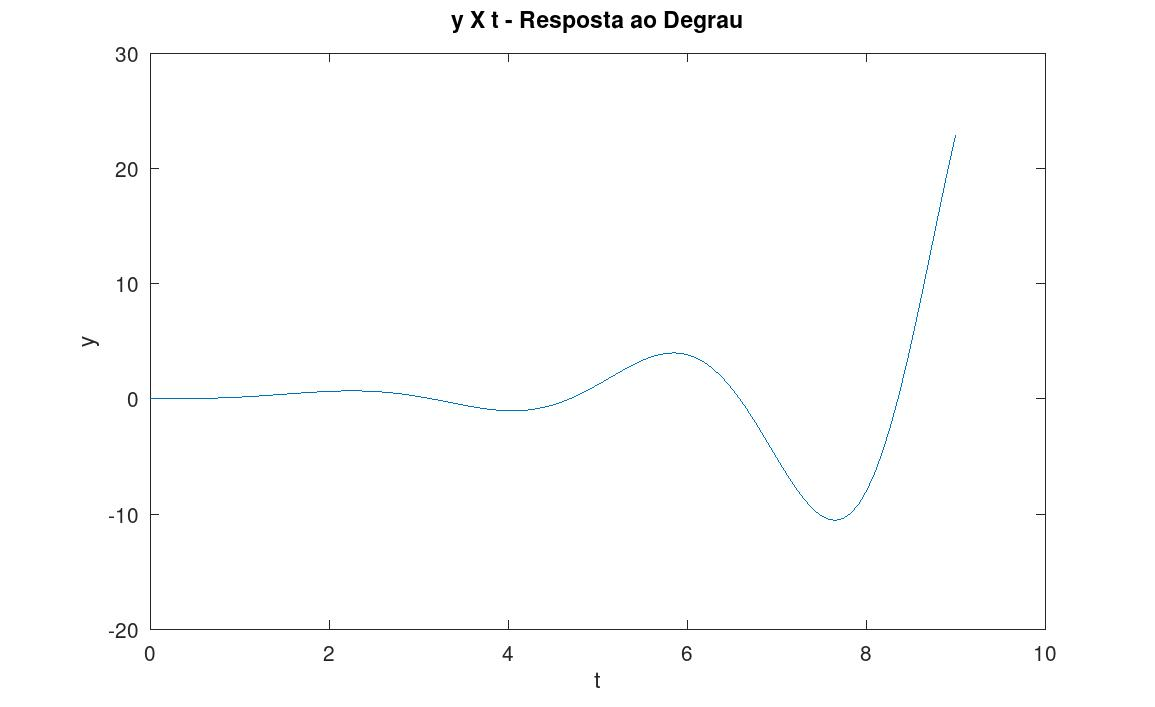
\includegraphics[scale=0.3]{plot1c1.jpg}
\end{minipage}
\begin{minipage}[!]{0.5\linewidth}
  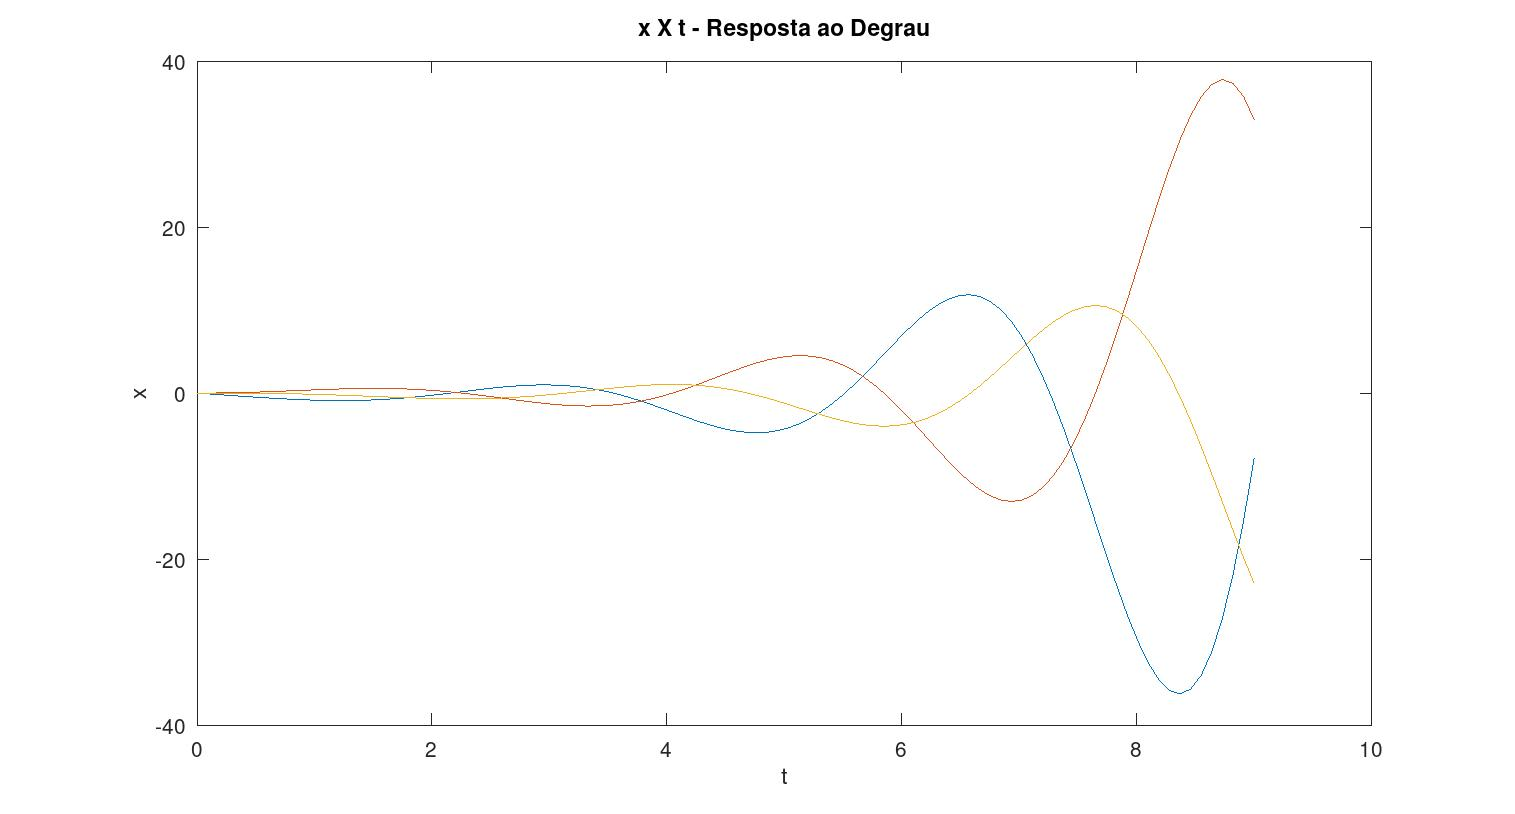
\includegraphics[scale=0.3]{plot1c2.jpg}
\end{minipage}
\end{figure}
\end{center}

\textbf{(d) encontre manualmente os autovetores;}

Vamos encontrar as raízes de $\Delta(s)$ que são os autovalores de $A$. Para isso, podemos utilizar a função \texttt{eig} no Octave para encontrá-los. Dessa forma, encontramos os seguintes valores:
\begin{align*}
  \lambda_1 &= -1.1795;\\
  \lambda_2 &= 0.5898 + j1.7445;\\
  \lambda_3 &= 0.5898 - j1.7445
\end{align*}

Chamando de $\lambda$ quaisquer uma das três raízes, teremos que:
\begin{align*}
  \begin{bmatrix}
    0 & 1 & 0\\
    0 & 0 & 1\\
    -4 & -2 & 0
  \end{bmatrix}
  \begin{bmatrix}
    \alpha\\
    \beta\\
    \gamma
  \end{bmatrix}
  =
  \lambda
  \begin{bmatrix}
    \alpha\\
    \beta\\
    \gamma
  \end{bmatrix}
\end{align*}

ou
\begin{align*}
  \begin{cases}
    \beta  &= \lambda \alpha\\
    \gamma &= \lambda \beta\\
    -4\alpha - 2\beta &= \lambda \gamma
  \end{cases}
  &
  &
  \begin{cases}
    \alpha &= \alpha\\
    \beta  &= \lambda \alpha\\
    \gamma &= \lambda^2 \alpha
  \end{cases}
\end{align*}

Ficamos, com um padrão para os autovetores:
\begin{align*}
  \alpha
  \begin{bmatrix}
    1\\
    \lambda\\
    \lambda^2
  \end{bmatrix}
\end{align*}

Temos, finalmente, como autovetores, os seguintes vetores:
\begin{align*}
  v_1 &=
  \begin{bmatrix}
    1\\
    -1.1795\\
    1.39122
  \end{bmatrix}
  &
  v_2 &=
  \begin{bmatrix}
    1\\
    0.5898 + j 1.7445\\
    -2.6954 + j 2.0578
  \end{bmatrix}
  &
  v_3 &=
  \begin{bmatrix}
    1\\
    0.5898 - j 1.7445\\
    -2.6954 - j 2.0578
  \end{bmatrix}
\end{align*}

\textbf{(e) escreva a REN seguindo o exemplo completo na nova versão dos slides094pwd.pdf a partir do slide 83;}

Sendo $v_1, v_2 \text{ e }, v_3$ os autovetores e $\lambda_1, \lambda_2, \lambda_3$ os autovalores, podemos  fazer uma pequena mudança para facilitar os cálculos, fazendo $\lambda_2 = \sigma + j\omega$ e $\lambda_3 = \sigma - j \omega$.
\begin{align*}
  x(t) &= \alpha v_1 e^{\lambda_1 t} + \beta v_2 e^{(\sigma + j\omega) t} + \gamma v_3 e^{(\sigma - j\omega) t}\\
       &= \alpha v_1 e^{\lambda_1 t} + \beta v_2 e^{\sigma t} e^{j \omega t} + \gamma v_3 e^{\sigma t} e^{-j \omega t}\\
       &= \alpha v_1 e^{\lambda_1 t} + \left[\beta v_2 e^{j \omega t} + \gamma v_3 e^{-j \omega t}\right] e^{\sigma t}\\
       &= \alpha v_1 e^{\lambda_1 t} + \left[(\beta v_2 + \gamma v_3) \cos(\omega t) + j(\beta v_2 - \gamma v_3) \sen(\omega t) \right] e^{\sigma t}
\end{align*}

Sabemos que $x(t)$ é real, então $(\beta v_2 + \gamma v_3)$ e $j(\beta v_2 - \gamma v_3)$ são reais.
\begin{align*}
  \beta v_2 + \gamma v_3 &=
  \begin{bmatrix}
    \beta + \gamma\\
    \sigma(\beta + \omega) + j\omega (\beta - \omega)\\
    (\sigma^2 - \omega^2)(\beta + \omega) + j 2 \sigma \omega (\beta - \omega)
  \end{bmatrix}
  &
  j(\beta v_2 - \gamma v_3) &=
  \begin{bmatrix}
    j(\beta - \gamma)\\
    j\sigma(\beta - \omega) - \omega (\beta + \omega)\\
    j(\sigma^2 - \omega^2)(\beta - \omega) - 2 \sigma \omega (\beta + \omega)
  \end{bmatrix}
\end{align*}

Fazendo $\beta + \gamma = \delta \in \mathbb{R}$ e $j(\beta - \gamma) = \epsilon \in \mathbb{R}$, teremos:
\begin{align*}
  \beta v_2 + \gamma v_3 &=
  \begin{bmatrix}
    \delta\\
    \sigma \delta + \omega \epsilon\\
    (\sigma^2 - \omega^2) \delta + 2 \sigma \omega \epsilon
  \end{bmatrix}
  &
  j(\beta v_2 - \gamma v_3) &=
  \begin{bmatrix}
    \epsilon\\
    \sigma \epsilon - \omega \delta\\
    (\sigma^2 - \omega^2) \epsilon - 2 \sigma \omega \delta
  \end{bmatrix}\\ %% ------------------------------------------
  \beta v_2 + \gamma v_3 &=
  \begin{bmatrix}
    1 & 0\\
    \sigma & \omega\\
    (\sigma^2 - \omega^2) & 2 \sigma \omega
  \end{bmatrix}
  \begin{bmatrix}
    \delta\\
    \epsilon
  \end{bmatrix}
  &
  j(\beta v_2 - \gamma v_3) &=
  \begin{bmatrix}
    1 & 0\\
    \sigma & \omega\\
    (\sigma^2 - \omega^2) & 2 \sigma \omega
  \end{bmatrix}
  \begin{bmatrix}
    \epsilon\\
    -\delta
  \end{bmatrix}
\end{align*}

Substituindo, teremos:
\begin{align*}
  x(t) = \alpha v_1 e^{\lambda_1 t} +
  \begin{bmatrix}
    1 & 0\\
    \sigma & \omega\\
    (\sigma^2 - \omega^2) & 2 \sigma \omega
  \end{bmatrix}
  \left\{
    \begin{bmatrix}
      \delta\\
      \epsilon
    \end{bmatrix}
    \cos(\omega t) +
    \begin{bmatrix}
      \epsilon\\
      -\delta
    \end{bmatrix}
    \sen(\omega t)
  \right\}
  e^{\sigma t}
\end{align*}

finalmente, tendo $\sigma = 0.5898$ e $\omega = 1.7445$.
\begin{align*}
  x(t) = \alpha
  \begin{bmatrix}
    1\\
    -1.1795\\
    1.39122
  \end{bmatrix}
  e^{-1.1795 t} + 
  \begin{bmatrix}
    1 & 0\\
    0.5898 & 1.7445\\
    -2.6954& 2.0578122
  \end{bmatrix}
  \left\{
    \begin{bmatrix}
      \delta\\
      \epsilon
    \end{bmatrix}
    \cos(1.7445 t) +
    \begin{bmatrix}
      \epsilon\\
      -\delta
    \end{bmatrix}
    \sen(1.7445 t)
  \right\}
  e^{0.5898 t}
\end{align*}

\textbf{(f) usando o comando \texttt{initial} encontre a REN ($y \text{ e } x$) para $x_0$ colocado em um ponto da matriz $V$;}

De maneira similar ao comando \texttt{step}, traremos os outputs \texttt{X, Y} do comando \texttt{initial}. Fazendo $\alpha = 1$ na equação $x(t)$.
\begin{verbatim}
... %% Programa anterior
%% REN
%% x0 como multiplo de V:
lambda1 = eig(A)(1)
x0_1 = [1 ; lambda1 ; lambda1^2]    %% Multiplo de V
[Y_ren_v, T_ren_v, X_ren_v] = initial(sp, x0_1)

%% Plotagem
plot(T_ren_v, Y_ren_v, "r", "linewidth", 3)
title("Y x T - REN (x0 = \lambda V)")
xlabel("t"), ylabel("y")

plot(T_ren_v, X_ren_v, "linewidth", 3)
title("X x T - REN (x0 = \lambda V)")
xlabel("t"), ylabel("x")
\end{verbatim}

Temos, por final, os gráficos:
\begin{center}
  \begin{figure}[h]
  \begin{minipage}[!]{0.5\linewidth}
    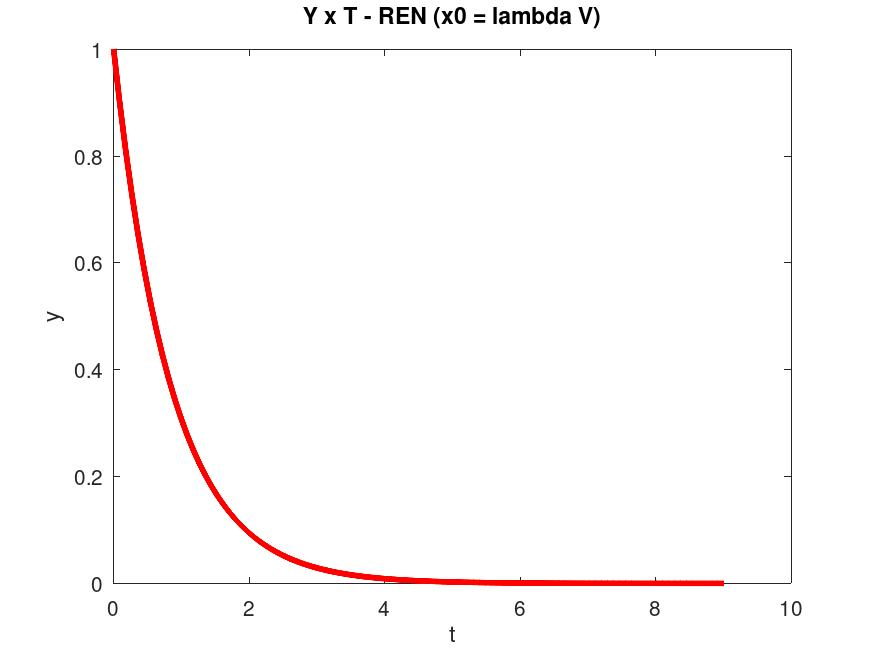
\includegraphics[scale=0.3]{plot1f1.jpg}
  \end{minipage}
  \begin{minipage}[!]{0.5\linewidth}
    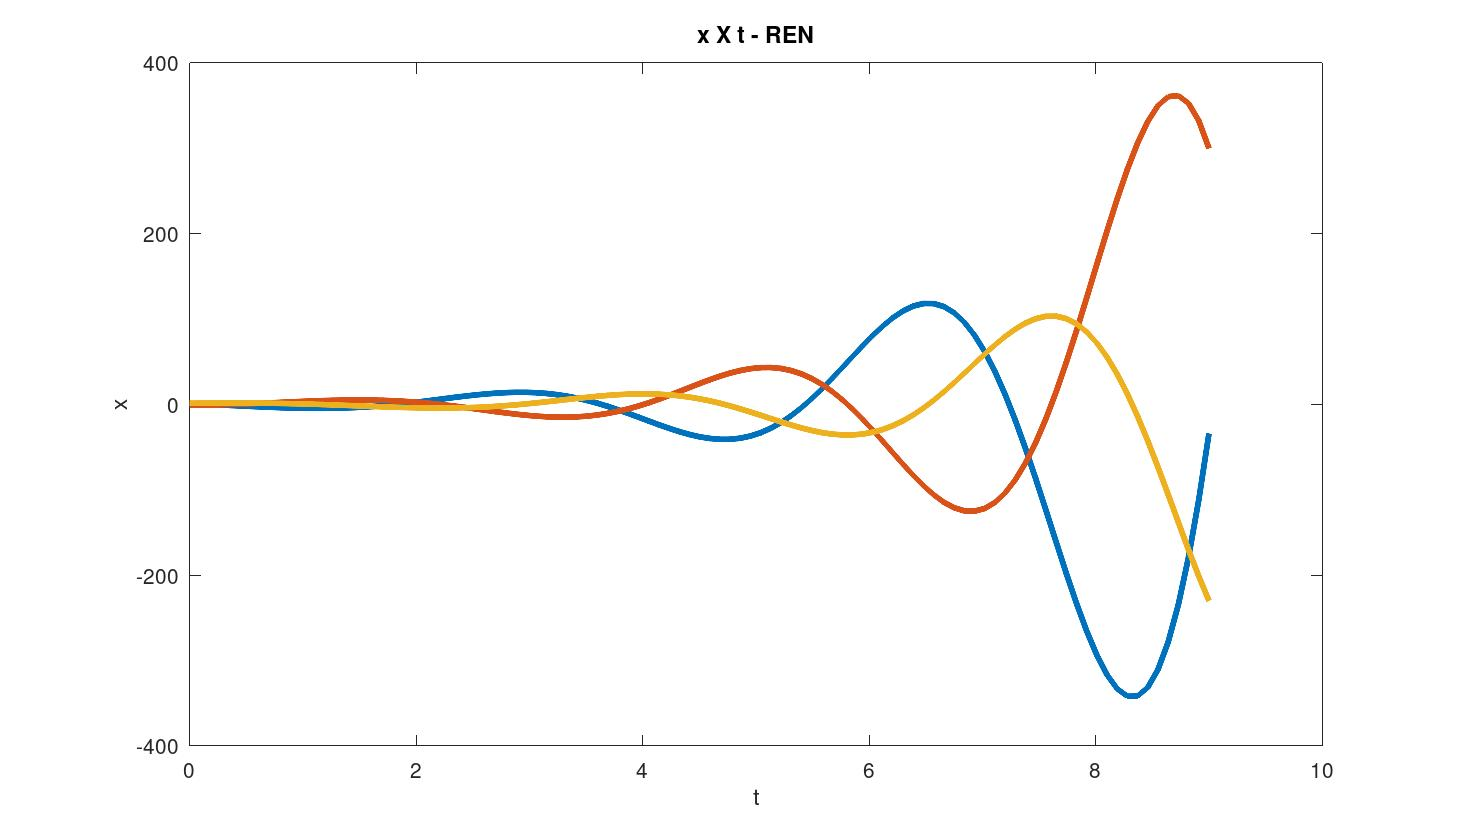
\includegraphics[scale=0.3]{plot1f2.jpg}
  \end{minipage}
  \end{figure}
\end{center}
\textbf{(g) idem para $x_0$ como uma combinação linear das colunas da matriz $W$.}

\begin{verbatim}
%% ... Programa anterior
%% REN
%% x0 como multiplo das colunas de W:
sigma = (eig(A)(2) + eig(A)(3)) / 2       %% Parte real
omega = (eig(A)(2) - eig(A)(3)) / (2 * i) %% Parte imaginaria
x0_2 = [1 ; sigma + omega ; (sigma^2 - omega^2) + 2 * sigma * omega]
[Y_ren_w, T_ren_w, X_ren_w] = initial(sp, x0_2)

%% Plotagem
%plot(T_ren_w, Y_ren_w, "r", "linewidth", 3)
title("Y x T - REN (x0 = C.L de W)")
xlabel("t"), ylabel("y")

%plot(T_ren_w, X_ren_w, "linewidth", 3)
title("X x T - REN (x0 = C.L de W)")
xlabel("t"), ylabel("x")
\end{verbatim}

Disso, obtemos:
\begin{center}
  \begin{figure}[h]
  \begin{minipage}[!]{0.5\linewidth}
    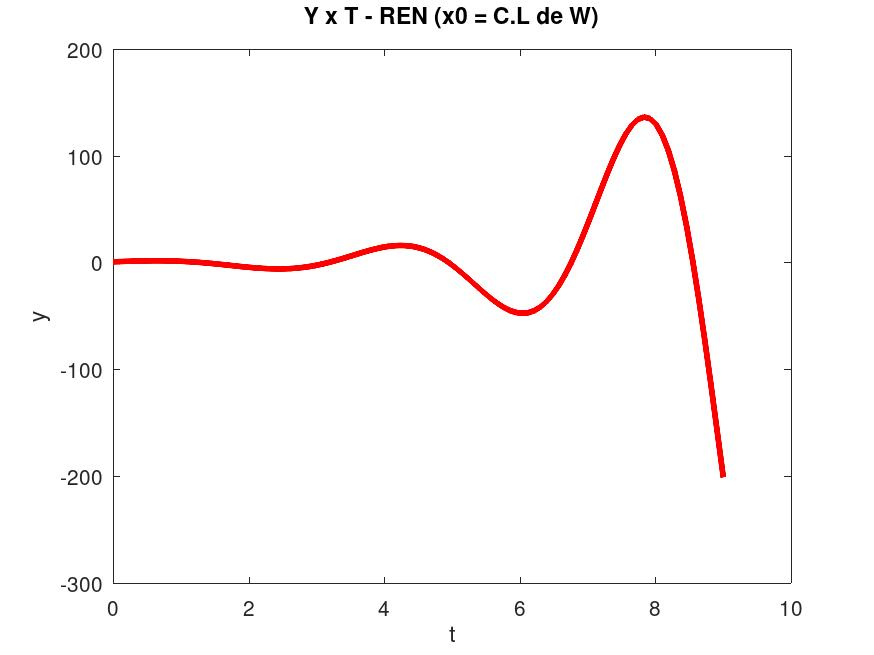
\includegraphics[scale=0.3]{plot1g1.jpg}
  \end{minipage}
  \begin{minipage}[!]{0.5\linewidth}
    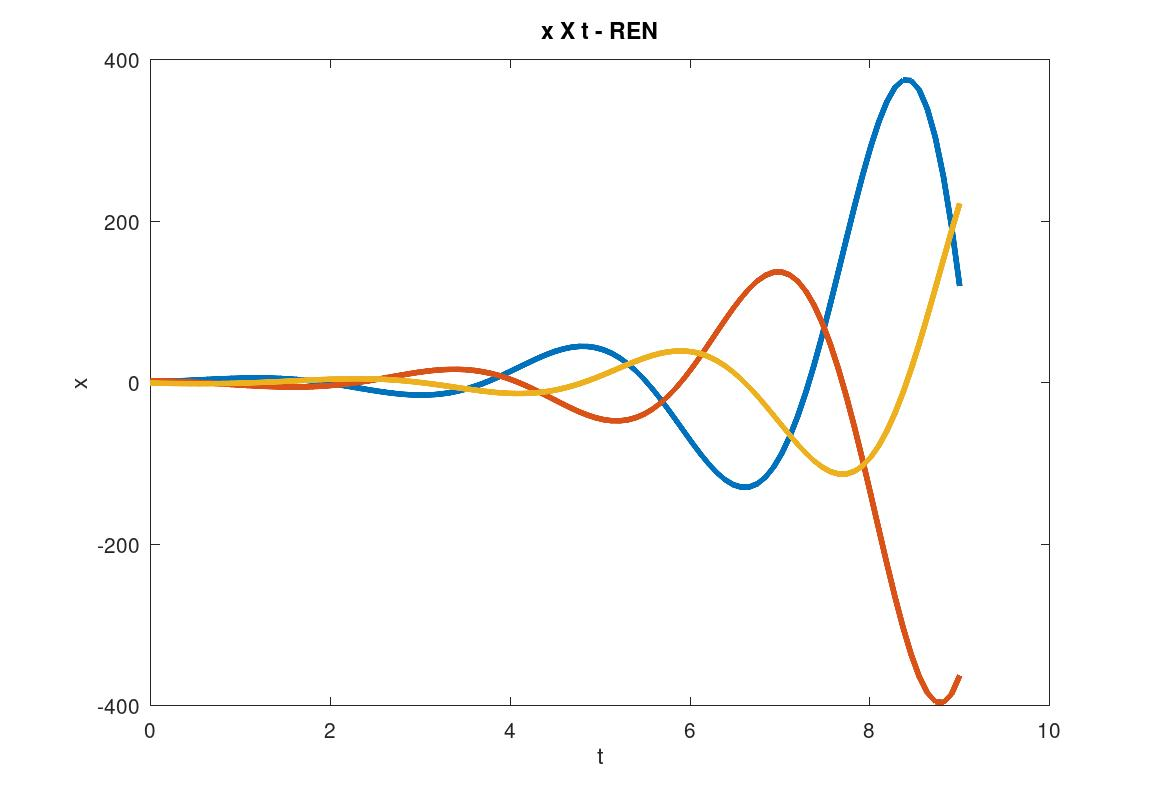
\includegraphics[scale=0.3]{plot1g2.jpg}
  \end{minipage}
  \end{figure}
\end{center}


%% ------------------------------------------------ %%
\textbf{2.) Um oscilador ideal com duas massas, molas e sem atritos e/ou amortecimentos é descrito por $\ddot{y_1}(t) + 2\omega_1^2 y_1(t) = \omega_1^2 y_2(t)$ e $\ddot{y_2}(t) + 2\omega_2^2 y_2(t) = \omega_2^2 y_1(t)$. Use a escolha $x_1 = y_1; x_2 = \dot{y_1}; x_3 = y_2; x_4 = \dot{y_2}$ para variáveis de estado, ou qualquer outra, e considere $\omega_1 = \omega_2 = \omega_0$.}

\textbf{G2: } $\omega_0 = 2$.

\textbf{(a) Encontre a matriz de estados $A$, seu polinômio característico $\Delta(s)$;}
\[\ddot{y_1}(t) + 8 y_1(t) = 4 y_2(t) ; \ddot{y_2}(t) + 8 y_2(t) = 4 y_1(t)\]
\[x_1 = y_1; x_2 = \dot{y_1}; x_3 = y_2; x_4 = \dot{y_2}\]
\[\dot{x_1}(t) = \dot{y_1}(t) = x_2(t)\]
\[\dot{x_2}(t) = \ddot{y_1}(t) = - 8 y_1(t) + 4 y_2(t) = - 8 x_1 + 4 x_3\]
\[\dot{x_3}(t) = \dot{y_2}(t) = x_4\]
\[\dot{x_4}(t) = \ddot{y_2}(t) = 4 y_1(t) - 8 y_2(t) = 4 x_1 - 8 x_3\]
\[A = \left[ {\begin{array}{cccc}
  0 & 1 & 0 & 0 \\
  -8 & 0 & 4 & 0 \\
  0 & 0 & 0 & 1 \\
  4 & 0 & -8 & 0 \\
\end{array} } \right]\]
\[
\Delta(s) = det(sI - A) = det\left(
\left[ {\begin{array}{cccc}
  s & 0 & 0 & 0 \\
  0 & s & 0 & 0 \\
  0 & 0 & s & 0 \\
  0 & 0 & 0 & s \\
\end{array} } \right]
-
\left[ {\begin{array}{cccc}
  0 & 1 & 0 & 0 \\
  -8 & 0 & 4 & 0 \\
  0 & 0 & 0 & 1 \\
  4 & 0 & -8 & 0 \\
  \end{array} } \right]
  \right)
  =
  \left| \begin{array}{cccc}
    s & -1  & 0 &  0\\ 
    8 & s & -4 & 0 \\
    0 & 0  & s & -1 \\
    -4 & 0  & 8 & s \\
  \end{array}
  \right|
  = s^4 + 16s^2 + 48
\]

\textbf{(b) os autovalores (faça $\lambda_1; \lambda_2; \lambda_3; \lambda_4;$ pares complexos conjugados) e, manualmente, os autovetores $v_1, v_2, v_3, v_4$;}
Vamos encontrar as raízes de $\Delta(s)$ que são os autovalores de $A$. Para isso, podemos utilizar a função \texttt{eig} no Octave para encontrá-los. Dessa forma, encontramos os seguintes valores:
\[
  \lambda_1 = 2j; \lambda_2 = -2j; \lambda_3 = 2\sqrt{3}j; \lambda_4 = -2\sqrt{3}j
\]
Chamando de $\lambda$ quaisquer uma das quatro raízes, teremos que:
\begin{align*}
  \begin{bmatrix}
    0 & 1 & 0 & 0 \\
    -8 & 0 & 4 & 0 \\
    0 & 0 & 0 & 1 \\
    4 & 0 & -8 & 0 \\
  \end{bmatrix}
  \begin{bmatrix}
    \alpha\\
    \beta\\
    \gamma\\
    \delta
  \end{bmatrix}
  =
  \lambda
  \begin{bmatrix}
    \alpha\\
    \beta\\
    \gamma\\
    \delta
  \end{bmatrix}
\end{align*}
ou
\begin{align*}
  \begin{cases}
    \beta  &= \lambda \alpha\\
    -8\alpha + 4\gamma &= \lambda \beta\\
    \delta &= \lambda \gamma \\
    4\alpha - 8\gamma &= \lambda \delta
  \end{cases}
  &
  &
  \begin{cases}
    \alpha &= \alpha\\
    \beta  &= \alpha \lambda\\
    \gamma &= \frac{\alpha (\lambda^2 +8)}{4} \\
    \delta &= \frac{\alpha (\lambda^3 + \lambda 8)}{4}
  \end{cases}
\end{align*}
Ficamos, com um padrão para os autovetores:
\begin{align*}
  \alpha
  \begin{bmatrix}
    1\\
    \lambda\\
    \frac{\lambda^2 +8}{4} \\
    \frac{\lambda^3 +\lambda 8}{4}
  \end{bmatrix}
\end{align*}
Temos, finalmente, como autovetores, os seguintes vetores:
\begin{align*}
  v_1 &=
  \begin{bmatrix}
    1\\
    2j\\
    1\\
    2j
  \end{bmatrix}
  &
  v_2 &=
  \begin{bmatrix}
    1\\
    -2j\\
    1\\
    -2j
  \end{bmatrix}
  &
  v_3 &=
  \begin{bmatrix}
    1\\
    2\sqrt{3}j\\
    -1\\
    -2\sqrt{3}j
  \end{bmatrix}
  &
  v_4 &=
  \begin{bmatrix}
    1\\
    -2\sqrt{3}j\\
    -1\\
    2\sqrt{3}j
  \end{bmatrix}
\end{align*}

\textbf{(c) escreva a expressão da REN: $x(t) = \sum_{i=1}^{4} r_i v_i e^{\lambda_i t}$ onde os $r_i$ são parâmetros de cada modo e os $\lambda_i$ são os autovalores;}

\begin{align*}
  x(t) = \sum_{i=1}^{4} r_i v_i e^{\lambda_i t} =
  r_1
  \begin{bmatrix}
    1\\
    2j\\
    1\\
    2j
  \end{bmatrix}
  e^{2j t} +
  r_2
  \begin{bmatrix}
    1\\
    -2j\\
    1\\
    -2j
  \end{bmatrix}
  e^{-2j t} +
  r_3
  \begin{bmatrix}
    1\\
    2\sqrt{3}j\\
    -1\\
    -2\sqrt{3}j
  \end{bmatrix}
  e^{2\sqrt{3}j t} +
  r_4
  \begin{bmatrix}
    1\\
    -2\sqrt{3}j\\
    -1\\
    2\sqrt{3}j
  \end{bmatrix}
  e^{-2\sqrt{3}j t}
\end{align*}

\textbf{(d) usando a identidade de Euler, coloque a expressão acima em uma forma onde apareçam senos e co-seno;}

Sabemos que a identidade de Euler é dada por:
\begin{align*}
  e^{j\theta} = cos(\theta) + jsen(\theta)
\end{align*}

Ao aplicar na expressão da questão anterior, obtemos:
\[V_1(\cos(2t)+j\sen(2t)) \, +\]
\[V_2(\cos(-2t)-j\sen(2t)) \, +\]
\[V_3(\cos(2\sqrt{3}t)+j\sen(2\sqrt{3}t)) \, +\]
\[V_4(\cos(-2\sqrt{3}t)-j\sen(2\sqrt{3}t)) \, =\]
\[(V_1+V_2)\cos(2t) + (V_1-V_2)j\sen(2t) + (V_3+V_4)cos(2\sqrt{3}t) + (V_3-V_4)jsen(2\sqrt{3}t)\]

Finalmente:
\begin{align*}
  x(t) =
  \begin{bmatrix}
    r_1+r_2\\
    2j(r_1-r_2)\\
    r_1+r_2\\
    2j(r_1-r_2)
  \end{bmatrix}
  cos(2t) +
    \begin{bmatrix}
      r_1-r_2\\
      2j(r_1+r_2)\\
      r_1-r_2\\
      2j(r_1+r_2)
    \end{bmatrix}
    jsen(2t) + \\
  \begin{bmatrix}
    r_3+r_4\\
    2\sqrt{3}j(r_3-r_4)\\
    -r_3-r_4\\
    -2\sqrt{3}j(r_3-r_4)
  \end{bmatrix}
  cos(2\sqrt{3}t) +
  \begin{bmatrix}
    r_3-r_4\\
    2\sqrt{3}j(r_3+r_4)\\
    -r_3+r_4\\
    -2\sqrt{3}j(r_3+r_4)
  \end{bmatrix}
  jsen(2\sqrt{3}t)
\end{align*}

\textbf{(e) analisando esta última expressão, verifique que os pares $r_1 \text{ e } r_2, r_3 \text{ e } r_4$ são complexos conjugados;}

Primeiramente, vamos relembrar do que se trata a equação acima.

$x(t) = \sum_{i=1}^4 r_i v_i e^{\lambda_i t}$, é a expressão da REN de um sistema massa mola.

Isso significa que a equação representa um sistema físico, e portanto, as somas e variáveis das componentes de $x(t)$ devem ser Reais.

Vamos analisar esta primeira parcela da equação da questão anterior:

\begin{align*}
  \begin{bmatrix}
    r_1+r_2\\
    2j(r_1-r_2)\\
    r_1+r_2\\
    2j(r_1-r_2)
  \end{bmatrix}
  cos(2t)
\end{align*}

Observe que, para que o produto de cada termo desse vetor pelo $cos(2t)$ resulte em um número Real, os pares $r_1 \text{ e } r_2, r_3 \text{ e } r_4$ devem obedecer à seguinte relação:\
$r_1+r_2$ resulta em um número Real, pois $cos(2t)$ também é um Real.\
$r_1-r_2$ resulta em um número Imaginário puro, devido ao termo $2j$.\
Analogamente, para os termos $r_3\ e\ r_4$, chegamos à conclusão final de que:\
$r_1+r_2$ e $r_3+r_4$ são números Reais.\
$r_1-r_2$ e $r_3-r_4$ são números Imaginários.\
Com isso, as condições acima mostram que $r_1 \text{ e } r_2, r_3 \text{ e } r_4$ formam pares complexos conjugados.\

\textbf{(f) usando $r_1 = \alpha + j\beta, r_2 = \alpha - j\beta$, $r_3 = \gamma + j\delta, r_4 = \gamma - j\delta$ encontre a expressão final para $x(t)$;}
\begin{align*}
  x(t) =
  \begin{bmatrix}
    2\alpha\\
    -4\beta\\
    2\alpha\\
    -4\beta
  \end{bmatrix}
  \cos(2t) +
  \begin{bmatrix}
    -2\beta\\
    -4\alpha\\
    -2\beta\\
    -4\alpha
  \end{bmatrix}
  \sen(2t) +
  \begin{bmatrix}
    2\gamma\\
    -4\sqrt{3}\delta\\
    -2\gamma\\
    4\sqrt{3}\delta
  \end{bmatrix}
  \cos(2\sqrt{3}t) +
  \begin{bmatrix}
    -2\delta\\
    -4\sqrt{3}\gamma\\
    2\delta\\
    4\sqrt{3}\gamma
  \end{bmatrix}
  \sen(2\sqrt{3}t)
\end{align*}

Reescrenvendo, temos:
\begin{align*}
  x(t) =
  \begin{bmatrix}
    2 & 0\\
    0 & -4\\
    2 & 0\\
    0 & -4
  \end{bmatrix}
  \left[
    \begin{bmatrix}
      \alpha\\
      \beta
    \end{bmatrix}
    \cos(2t) +
    \begin{bmatrix}
      -\beta\\
      \alpha
    \end{bmatrix}
    \sen(2t)
  \right] + 
  \begin{bmatrix}
    2 & 0\\
    0 & -4\sqrt{3}\\
    -2 & 0\\
    0 & 4\sqrt{3}
  \end{bmatrix}
  \left[
    \begin{bmatrix}
      \gamma\\
      \delta
    \end{bmatrix}
    \cos(2\sqrt{3}t) +
    \begin{bmatrix}
      -\delta\\
      \gamma
    \end{bmatrix}
    \sen(2\sqrt{3}t)
  \right]
\end{align*}

\textbf{(g) encontre o estado inicial $x_0$ que corresponde a $(\alpha, \beta, \gamma, \delta) = (1, 0, 0, 0)$ e plote $x(t)$ no Octave (comando \texttt{initial});}

\begin{align*}
  x(0) =
  \begin{bmatrix}
    2\alpha\\
    -4\beta\\
    2\alpha\\
    -4\beta
  \end{bmatrix}
  +
  \begin{bmatrix}
    2\gamma\\
    -4\sqrt{3}\delta\\
    -2\gamma\\
    4\sqrt{3}\delta
  \end{bmatrix}
  =
  \begin{bmatrix}
    2\alpha + 2\gamma\\
    -4\beta - 4\sqrt{3}\delta\\
    2\alpha - 2\gamma\\
    -4\beta + 4\sqrt{3}\delta
  \end{bmatrix}
\end{align*}

\begin{align*}
  x(0) =
  \begin{bmatrix}
    2 \\
    0\\
    2\\
    0
  \end{bmatrix}
  para (\alpha, \beta, \gamma, \delta) = (1, 0, 0, 0)
\end{align*}

\textbf{(h) idem $(\alpha, \beta, \gamma, \delta) = (0, 0, 1, 0)$ idem;}

\begin{align*}
  x(0) =
  \begin{bmatrix}
    2 \\
    0\\
    -2\\
    0
  \end{bmatrix}
\end{align*}

\textbf{(i) idem $(\alpha, \beta, \gamma, \delta) = (1, 0, 1, 0)$ idem;}

\begin{align*}
  x(0) =
  \begin{bmatrix}
    4 \\
    0\\
    0\\
    0
  \end{bmatrix}
\end{align*}

\textbf{(j) idem $(\alpha, \beta, \gamma, \delta) = $ sua escolha idem;}

\textbf{(k) comente as curvas obtidas.}

\end{document}